\chapter{Theoretischer Rahmen}
\section{Spaced Repetition}
Gespeicherte Informationen können in zwei Kategorien eingeteilt werden. Bei der  \textit{familarity}-Darstellung kann sich an die Information erinnert werden, diese aber nicht in Kontext mit den dazugehörigen Informationen gebracht werden. Ein bekanntes Beispiel dazu wäre, dass einem bekannten Gesicht kein Namen zuordnen werden kann. Die andere Möglichkeit ist die \textit{recollection}-Darstellung, bei welcher sich auch an den jeweiligen Kontext erinnert werden kann. Angewendet auf das vorherige Beispiel, kann sich in diesen Fall an den Namen und weitere personenbezogene Informationen erinnert werden.\cite{SA:Forget}

Beide Darstellungen von Informationen werden im Gehirn durch Neuronen gespeichert. Durch Assoziationen werden die Neuronen mithilfe von synaptischen Verbindungen angeregt. Die Assoziationen sind bei jeder Erinnerung unterschiedlich und können von Farben und Tönen bis zu mathematischen Formeln gehen. Eine synaptische Verbindung ist nicht statisch und kann im Laufe der Zeit stärker und schwächer werden. Dazu kommt noch, dass Neuronen, die andere Neuronen aktivieren, mit der Zeit besser darin werden.\cite{SDW:Vergessen}

Wenn der Übertragungsmechanismus zu schwach wird, dann vergessen wir die Information. Die \textit{familarity}-Darstellung wird durch einen Prozess \textit{interference} (zu deutsch Störung oder Interferenz) vergessen. Dabei wird die Verbindung erschwert, indem gleiche Informationen oder Informationen mit gleichen Kontext hinzugefügt werden. Möglicherweise wird die bestehende Information sogar komplett überschrieben. \textit{Decay} (zu deutsch Verfall) heißt der Prozess, bei dem \textit{recollection}-Informationen vergessen werden. Dabei wird, wie der Name schon nahe legt, die synaptische Verbindung durch das seltene Benutzten so schwach, dass das Anregen der zugehörigen Neuronen zu stark erschwert wurde. Ganz verschwinden synaptischen Verbindungen nie, denn Gehirnanalysen zeigen, dass die Verbindungen auch nach größeren Zeiträumen ohne Nutzung weiter bestehen bleiben. Nach dieser Erkenntnis wird bei \textit{decay} metaphorisch davon gesprochen, dass der Schlüssel zum Safe mit den Informationen verlegt wurde.\cite{SA:Forget}\cite{SDW:Vergessen}

Der Vergessensprozess rührt aus der biologischen Natur des Menschen. Das Überschreiben von alten Informationen ermöglicht es dem Menschen flexibel zu sein und sich an neue Bedingungen anzupassen. Dazu kommt noch, dass da Gehirn als eine Art Spamfilter fungiert. Es filtert irrelevant Informationen aus und schützt so vor einem Informationsüberfluss. Ohne den könnte man sich daran erinnern, wo das Auto vor einer Woche oder einen Monat stand. Dadurch wird präzise und schnelle Informationsverarbeitung verhindert, da mehr Erinnerungen basierend auf einer Assoziation durchsucht werden müssen.\cite{SDW:Vergessen}

\subsection{Ebbinghaus's Forgetting Curve}
Durch Selbstversuche hat der deutsche Psychologe Hermann Ebbinghaus die Erinnerungsleistung des Gehirns studiert. Aus den Testergebnissen entstand die ebbinghaussche Vergessenskurve. Die Vergessenskurve ist ein viel genutztes Modell, um den Verfall von Informationen zu visualisieren. Sie beschreibt die Menge an gespeichertem Wissen relativ zur vergangenen Zeit, nachdem das zu erlernende Wissen das erste Mal fehlerfrei wiedergegeben wurde.\cite{Wiki:Vergessenskurve}

\begin{center}
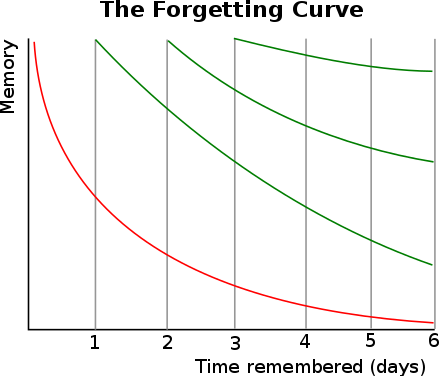
\includegraphics[width=0.4\textwidth]{images/vergessenskurve.png}
\end{center}

Auffällig an dem Modell ist die exponentiell ähnliche Abnahmen des erlangten Wissens. Die rote Kurve beschreibt den Anteil an gespeichertem Wissen ohne eine weitere Wiederholung. Ebbinghaus hält fest, dass er nach 20 Minuten nur noch in der Lage war, 60\% richtig wiederzugeben. Nach einer Stunde waren es noch 45\%. Einen Tag und sechs Tage danach lag das gemerkte Wissen nur noch bei 34\% bzw. 23\%. Über einen langen Zeitraum festigen sich nur 15\% des geübten Wissens. Wird der Lernprozess durch Wiederholungen (grüne Graphen) ergänzt, festigt sich das Thema mit der Zeit. Die Kurve flacht schneller ab und ist generell weniger steil.\cite{Wiki:Vergessenskurve}

Kritisiert wird das Modell von Forschern in Hinsicht auf das Selbstexperiment. Es wird hinterfragt, wie geeignet ein Selbstexperiment ist und inwiefern äußere Ereignisse Einfluss auf das Ergebnis hatten. Das Ebbinghaus sinnlose Silbenreihen genutzt hat, wird ebenfalls kritisiert, da Neurologie und Gehirnforschung gezeigt haben, dass persönlich bedeutsame Themen anderen Vergessenskurven unterliegen. Damit wurde bewiesen, dass Vergessen abhängig vom zu verinnerlichen Wissen ist, was in den Selbstversuchen nicht berücksichtigt wurde. Christian Michel und Felix Novak haben in neuen Studien diese Komponente berücksichtigt und den Anteil an vergessenem Wissen nach 5 Tagen und 30 Tagen festgehalten. Am geringsten wurden Prinzipien und Gesetzmäßigkeiten vergessen (1\% bzw. 5\% wurden vergessen). Gedichte konnten zu 75\% bzw. 50\% nach verstrichener Zeit wiedergegeben werden. 53\% bzw. 60\% der Prosa wurden vergessen. Die von Ebbinghaus genutzten sinnlosen Silbenreihen werden am schnellsten Vergessen. Nach der Zeit konnten lediglich 22\% bzw. 20\% richtig wiedergegeben werden.\cite{Wiki:Vergessenskurve}

Trotz der Kritik ist das Modell von Ebbinghaus eine gute Orientierung für den Prozess des Vergessens. Besonders, weil Schüler ein Spektrum an unterschiedlichen Dingen lernen müssen. Da es sich nicht lohnt, für alle Möglichkeiten unterschiedliche Vergessenskurven als Grundlage zu nehmen und die Fälle für ein Programm schwer zu unterscheiden sind, sollte von dem schlechtesten Fall ausgegangen werden.

\subsection{Konzept von Spaced Repetition}
Nach der Entdeckung der ebbinghausschen Vergessenskurve folgt Ansätze für ein darauf basierendes Lernverfahren. 

Bei \textit{Spaced Repetition} wird der Inhalt in gezielten Abständen wiederholt. Die anfängliche Idee war es, Karteikarten in Boxen zu kategorisieren. Die Boxen wurden von eins bis fünf durchnummeriert. Die Zahlen spiegeln den Fortschritt wieder. In der ersten Box sind die Karten, welche der Schüler am schlechtesten beherrscht. Wenn ein Schüler die Karteikarte erfolgreich wiedergeben kann, dann wird die Karte in die nächst höhere Box gelegt. Das bedeutet, im Fall einer Karte aus der Box eins wird diese in die Box 2 gelegt. Wenn eine Karte nicht wiedergegeben werden kann, dann wird diese egal wo sie vorher war, wieder in die Box eins gelegt. Beim lernen werden die Karten in der ersten Box priorisiert, um auf die Schwächen zu fokussieren. \par
Zu diesen Zeitpunkt hebt sich das Prinzip von \textit{Cramming} nicht gravierend von ab. Der essenzielle Part ist, dass die Boxen ständig um neue Karten erweitert und über einen langen Zeitraum geführt werden. Damit werden die Differenzen deutlich, da bei \textit{Cramming} alle wichtigen Informationen über wenige Tage mit dem einzigen Ziel für eine Klausur oder Abfrage zur Verfügung stehen. Die damit verbunden negativen Aspekte sind von der Hand zu weisen. Die Informationen stehen nur über einen kurzen Zeitraum zur Verfügung und werden schnell wieder vergessen. Das ist besonders kritisch, wenn andere Themen darauf aufbauen. Da alles vergessen

\subsection{Ergebnisse von Studien}
Es liegen diverse Studien vor, welche die Effektivität von \textit{Spaced Repetiton} analysieren und bestätigen. Dabei fächern sich die Beweismethoden auf verschiedene Bereiche. Bei Gehirnscans wird die Stärke von synaptischen Verbindungen untersucht. Andere Methoden sind auch Studien mit Probanden, durch welche unterschiedliche Lernmethoden verglichen werden.

Alison Voice von der University of Leeds und Arran Stirton von der University of Leicester haben in ihrer Studie \textit{Spaced Repetition: towards more effective learning in STEM} eine \textit{Spaced Repetition Software} für die Probanden entwickelt und die Auswirkungen auf das Prüfungsergebnis analysiert. Dafür wurde den neuen Thermodynamik-Studenten die Software direkt nach Start, 1/6 und 2/6 des Jahres vorgestellt. Dazu wurde mit irregulären Erinnerungen über das Jahr verteilt auf die Anwendung aufmerksam gemacht. Neben der Applikation konnten die Schüler lernen, wie sie wollten. Am Ende des Lehrjahres folgte eine Prüfung des Lernstands. Anschließend wurden die Testergebnisse verglichen. Während in dem ersten Jahr kein signifikant besseres Ergebnis der App-Nutzer gegenüber den nicht App-Nutzer erkennbar ist. Schnitten die App-Nutzer in den Jahrgängen 17-18 und 18-19 deutlich besser ab. Ergänzend zur Prüfung folgte nach den Ferien ein unangekündigter Test, mit welchen das Langzeitpotenzial getestet wurde. Generell schnitten die Schüler schlechter ab als in der Prüfung vor den Ferien, was mit dem Prinzip der ebbinghausschen Vergessenskurve übereinstimmt. Im Vergleich zwischen Nutzern und Nichtnutzern zeigten die Nutzer ein signifikant höheres Ergebnis, was das Langzeitpotenzial von \textit{Spaced Repetition} bestätigt.\cite{RD:SpacedRepetition}

Die Studie von Enikö A. Kramár und Kollegen untersucht die Stärke der Synapsenverbindungen in Hinblick auf das Langzeitpotenzial. Dafür wurden Synapsen eines Rattenhippocampus mit zwei \textit{Theta-Burst-Stimulationen} angeregt. Nach regelmäßigen Abständen wird die ursprüngliche Verbindung neu stimuliert. Dabei ging eine Steigerung Potenzierung nach 60 und 90 Minuten hervor. Eine erneute Stimulierung nach 10 oder 20 Minuten hat eine vergleichsweise minimale Steigerung. Des Weiteren hat die Studie festgestellt, dass eine dritte und vierte \textit{Theta-Burst-Stimulation} nach jeweiligen 60 Minuten kaum bis keine Auswirkungen auf die Langzeitpotenzierung hat, was einen steigenden Wiederholungsintervall impliziert. Ein Anstieg an Synapsen konnte von den Forschern ebenfalls nachgewiesen werden.\cite{PNAS:Synaptic}

\section{Dart und Flutter}
Dart ist eine von Google entwickelte Programmiersprache, welche auf Anwendungsentwicklung fokussiert ist, aber auch für Server genutzt werden kann. Anwendungen, die mit Dart programmiert werden, können Mobile Applikationen, Webseiten oder Desktop-Anwendungen sein. Die Syntax von Dart hat Ähnlichkeiten mit der Syntax von C. Dart implementiert viele herkömmliche Programmierpraktiken, wie Objektorientierung, Klassen und automatisierter Garbage Collection. 
Dart erschien erstmals am 10 Oktober 2011\par

Flutter ist eine SDK für Mobile Applikationen mit einem kompletten Framework und vorgefertigten Widgets und Tools. Mit Flutter geschriebene Anwendungen lassen sich "ahead-of-time" kompilieren und sind nativ auf Android, sowie auf IOS.
